\documentclass[tikz,border=5pt]{standalone}
\usepackage{amsmath,amssymb}
\usetikzlibrary{arrows.meta}
\definecolor{curveblue}{HTML}{245C86}
\definecolor{accent}{HTML}{A65E2E}
\begin{document}
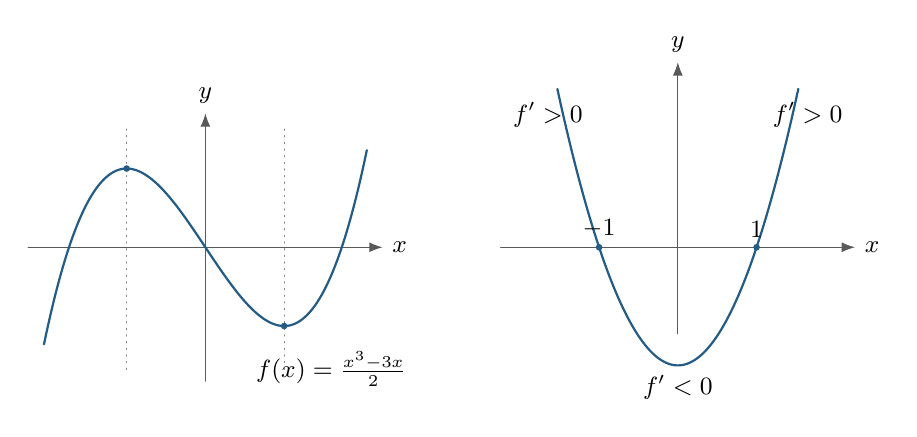
\begin{tikzpicture}[font=\small,>=Latex,line cap=round,line join=round]
\begin{scope}[shift={(0.00000,0.00000)},xscale=1,yscale=1]
\draw[->,black!65] (-2.25000,0.00000)--(2.25000,0.00000);
\node[right] at (2.25000,0.00000) {$x$};
\draw[->,black!65] (0.00000,-1.70000)--(0.00000,1.70000);
\node[above] at (0.00000,1.70000) {$y$};
\draw[curveblue,thick] plot[smooth] coordinates {(-2.05000,-1.23256) (-2.02267,-1.10355) (-1.99533,-0.97907) (-1.96800,-0.85906) (-1.94067,-0.74346) (-1.91333,-0.63221) (-1.88600,-0.52525) (-1.85867,-0.42251) (-1.83133,-0.32395) (-1.80400,-0.22948) (-1.77667,-0.13906) (-1.74933,-0.05263) (-1.72200,0.02989) (-1.69467,0.10855) (-1.66733,0.18341) (-1.64000,0.25453) (-1.61267,0.32197) (-1.58533,0.38581) (-1.55800,0.44608) (-1.53067,0.50287) (-1.50333,0.55622) (-1.47600,0.60621) (-1.44867,0.65289) (-1.42133,0.69632) (-1.39400,0.73656) (-1.36667,0.77369) (-1.33933,0.80774) (-1.31200,0.83880) (-1.28467,0.86691) (-1.25733,0.89215) (-1.23000,0.91457) (-1.20267,0.93423) (-1.17533,0.95119) (-1.14800,0.96552) (-1.12067,0.97728) (-1.09333,0.98653) (-1.06600,0.99332) (-1.03867,0.99773) (-1.01133,0.99981) (-0.98400,0.99962) (-0.95667,0.99722) (-0.92933,0.99269) (-0.90200,0.98606) (-0.87467,0.97742) (-0.84733,0.96682) (-0.82000,0.95432) (-0.79267,0.93998) (-0.76533,0.92386) (-0.73800,0.90603) (-0.71067,0.88654) (-0.68333,0.86546) (-0.65600,0.84285) (-0.62867,0.81877) (-0.60133,0.79328) (-0.57400,0.76644) (-0.54667,0.73832) (-0.51933,0.70897) (-0.49200,0.67845) (-0.46467,0.64684) (-0.43733,0.61418) (-0.41000,0.58054) (-0.38267,0.54598) (-0.35533,0.51057) (-0.32800,0.47436) (-0.30067,0.43741) (-0.27333,0.39979) (-0.24600,0.36156) (-0.21867,0.32277) (-0.19133,0.28350) (-0.16400,0.24379) (-0.13667,0.20372) (-0.10933,0.16335) (-0.08200,0.12272) (-0.05467,0.08192) (-0.02733,0.04099) (0.00000,0.00000) (0.02733,-0.04099) (0.05467,-0.08192) (0.08200,-0.12272) (0.10933,-0.16335) (0.13667,-0.20372) (0.16400,-0.24379) (0.19133,-0.28350) (0.21867,-0.32277) (0.24600,-0.36156) (0.27333,-0.39979) (0.30067,-0.43741) (0.32800,-0.47436) (0.35533,-0.51057) (0.38267,-0.54598) (0.41000,-0.58054) (0.43733,-0.61418) (0.46467,-0.64684) (0.49200,-0.67845) (0.51933,-0.70897) (0.54667,-0.73832) (0.57400,-0.76644) (0.60133,-0.79328) (0.62867,-0.81877) (0.65600,-0.84285) (0.68333,-0.86546) (0.71067,-0.88654) (0.73800,-0.90603) (0.76533,-0.92386) (0.79267,-0.93998) (0.82000,-0.95432) (0.84733,-0.96682) (0.87467,-0.97742) (0.90200,-0.98606) (0.92933,-0.99269) (0.95667,-0.99722) (0.98400,-0.99962) (1.01133,-0.99981) (1.03867,-0.99773) (1.06600,-0.99332) (1.09333,-0.98653) (1.12067,-0.97728) (1.14800,-0.96552) (1.17533,-0.95119) (1.20267,-0.93423) (1.23000,-0.91457) (1.25733,-0.89215) (1.28467,-0.86691) (1.31200,-0.83880) (1.33933,-0.80774) (1.36667,-0.77369) (1.39400,-0.73656) (1.42133,-0.69632) (1.44867,-0.65289) (1.47600,-0.60621) (1.50333,-0.55622) (1.53067,-0.50287) (1.55800,-0.44608) (1.58533,-0.38581) (1.61267,-0.32197) (1.64000,-0.25453) (1.66733,-0.18341) (1.69467,-0.10855) (1.72200,-0.02989) (1.74933,0.05263) (1.77667,0.13906) (1.80400,0.22948) (1.83133,0.32395) (1.85867,0.42251) (1.88600,0.52525) (1.91333,0.63221) (1.94067,0.74346) (1.96800,0.85906) (1.99533,0.97907) (2.02267,1.10355) (2.05000,1.23256)};
\draw[gray,dotted] (-1.00000,-1.55000)--(-1.00000,1.55000);
\fill[curveblue] (-1.00000,1.00000) circle (1.2pt);
\draw[gray,dotted] (1.00000,-1.55000)--(1.00000,1.55000);
\fill[curveblue] (1.00000,-1.00000) circle (1.2pt);
\node[below] at (1.60000,-1.20000) {$f(x)=\frac{x^3-3x}{2}$};
\end{scope}
\begin{scope}[shift={(6.00000,0.00000)},xscale=1,yscale=1]
\draw[->,black!65] (-2.25000,0.00000)--(2.25000,0.00000);
\node[right] at (2.25000,0.00000) {$x$};
\draw[->,black!65] (0.00000,-1.10000)--(0.00000,2.35000);
\node[above] at (0.00000,2.35000) {$y$};
\draw[curveblue,thick] plot[smooth] coordinates {(-1.53000,2.01135) (-1.50960,1.91834) (-1.48920,1.82657) (-1.46880,1.73606) (-1.44840,1.64679) (-1.42800,1.55878) (-1.40760,1.47201) (-1.38720,1.38649) (-1.36680,1.30221) (-1.34640,1.21919) (-1.32600,1.13741) (-1.30560,1.05689) (-1.28520,0.97761) (-1.26480,0.89958) (-1.24440,0.82280) (-1.22400,0.74726) (-1.20360,0.67298) (-1.18320,0.59994) (-1.16280,0.52816) (-1.14240,0.45762) (-1.12200,0.38833) (-1.10160,0.32028) (-1.08120,0.25349) (-1.06080,0.18794) (-1.04040,0.12365) (-1.02000,0.06060) (-0.99960,-0.00120) (-0.97920,-0.06175) (-0.95880,-0.12105) (-0.93840,-0.17911) (-0.91800,-0.23591) (-0.89760,-0.29147) (-0.87720,-0.34578) (-0.85680,-0.39884) (-0.83640,-0.45065) (-0.81600,-0.50122) (-0.79560,-0.55053) (-0.77520,-0.59860) (-0.75480,-0.64542) (-0.73440,-0.69098) (-0.71400,-0.73531) (-0.69360,-0.77838) (-0.67320,-0.82020) (-0.65280,-0.86078) (-0.63240,-0.90011) (-0.61200,-0.93818) (-0.59160,-0.97501) (-0.57120,-1.01060) (-0.55080,-1.04493) (-0.53040,-1.07801) (-0.51000,-1.10985) (-0.48960,-1.14044) (-0.46920,-1.16978) (-0.44880,-1.19787) (-0.42840,-1.22471) (-0.40800,-1.25030) (-0.38760,-1.27465) (-0.36720,-1.29775) (-0.34680,-1.31959) (-0.32640,-1.34019) (-0.30600,-1.35955) (-0.28560,-1.37765) (-0.26520,-1.39450) (-0.24480,-1.41011) (-0.22440,-1.42447) (-0.20400,-1.43758) (-0.18360,-1.44944) (-0.16320,-1.46005) (-0.14280,-1.46941) (-0.12240,-1.47753) (-0.10200,-1.48439) (-0.08160,-1.49001) (-0.06120,-1.49438) (-0.04080,-1.49750) (-0.02040,-1.49938) (0.00000,-1.50000) (0.02040,-1.49938) (0.04080,-1.49750) (0.06120,-1.49438) (0.08160,-1.49001) (0.10200,-1.48439) (0.12240,-1.47753) (0.14280,-1.46941) (0.16320,-1.46005) (0.18360,-1.44944) (0.20400,-1.43758) (0.22440,-1.42447) (0.24480,-1.41011) (0.26520,-1.39450) (0.28560,-1.37765) (0.30600,-1.35955) (0.32640,-1.34019) (0.34680,-1.31959) (0.36720,-1.29775) (0.38760,-1.27465) (0.40800,-1.25030) (0.42840,-1.22471) (0.44880,-1.19787) (0.46920,-1.16978) (0.48960,-1.14044) (0.51000,-1.10985) (0.53040,-1.07801) (0.55080,-1.04493) (0.57120,-1.01060) (0.59160,-0.97501) (0.61200,-0.93818) (0.63240,-0.90011) (0.65280,-0.86078) (0.67320,-0.82020) (0.69360,-0.77838) (0.71400,-0.73531) (0.73440,-0.69098) (0.75480,-0.64542) (0.77520,-0.59860) (0.79560,-0.55053) (0.81600,-0.50122) (0.83640,-0.45065) (0.85680,-0.39884) (0.87720,-0.34578) (0.89760,-0.29147) (0.91800,-0.23591) (0.93840,-0.17911) (0.95880,-0.12105) (0.97920,-0.06175) (0.99960,-0.00120) (1.02000,0.06060) (1.04040,0.12365) (1.06080,0.18794) (1.08120,0.25349) (1.10160,0.32028) (1.12200,0.38833) (1.14240,0.45762) (1.16280,0.52816) (1.18320,0.59994) (1.20360,0.67298) (1.22400,0.74726) (1.24440,0.82280) (1.26480,0.89958) (1.28520,0.97761) (1.30560,1.05689) (1.32600,1.13741) (1.34640,1.21919) (1.36680,1.30221) (1.38720,1.38649) (1.40760,1.47201) (1.42800,1.55878) (1.44840,1.64679) (1.46880,1.73606) (1.48920,1.82657) (1.50960,1.91834) (1.53000,2.01135)};
\fill[curveblue] (-1.00000,0.00000) circle (1.2pt);
\node[above] at (-1.00000,0.00000) {$-1$};
\fill[curveblue] (1.00000,0.00000) circle (1.2pt);
\node[above] at (1.00000,0.00000) {$1$};
\node[below] at (0.00000,-1.50000) {$f^{\prime}<0$};
\node[above] at (-1.65000,1.40000) {$f^{\prime}>0$};
\node[above] at (1.65000,1.40000) {$f^{\prime}>0$};
\end{scope}
\end{tikzpicture}
\end{document}
